% Proposal adapted to the official MDPI LaTeX article template.
% MDPI template source: https://www.mdpi.com/authors/latex
\documentclass[applsci,article,submit,oneauthor,pdftex]{Definitions/mdpi}
% MDPI loads hyperref via a begin-document hook; use the class's supported
% url-color command once the document starts.
\AtBeginDocument{\changeurlcolor{bluecite}}

% Additional packages used by the proposal body (the MDPI class loads the common packages).
\usepackage{mathtools}
\usepackage{listings}
\usepackage{pgfplots}
\pgfplotsset{compat=1.18}
\usetikzlibrary{arrows.meta,positioning,shapes.geometric,calc,fit}
\setlength{\headheight}{25pt}

% Project-specific notation, diagrams and code styling.
\definecolor{primary}{RGB}{20,60,120}
\definecolor{accent}{RGB}{0,120,180}
\definecolor{lightbg}{RGB}{247,249,252}
\definecolor{codebg}{RGB}{245,245,245}
\definecolor{codegreen}{RGB}{30,130,30}
\definecolor{codegray}{RGB}{120,120,120}
\definecolor{codepurple}{RGB}{130,0,160}
\definecolor{codeblue}{RGB}{0,0,200}
\definecolor{outputbg}{RGB}{240,248,240}
\definecolor{outputborder}{RGB}{100,160,100}
\definecolor{warningbg}{RGB}{255,250,230}
\definecolor{warningborder}{RGB}{200,160,40}
\definecolor{serverblue}{HTML}{1F4E79}
\definecolor{clientgreen}{HTML}{2E7D32}
\definecolor{accentorange}{HTML}{C75B12}
\definecolor{softgray}{HTML}{F5F7FA}


\lstdefinestyle{cstyle}{
  backgroundcolor=\color{codebg},
  commentstyle=\color{codegreen}\itshape\small,
  keywordstyle=\color{codeblue}\bfseries,
  numberstyle=\tiny\color{codegray},
  stringstyle=\color{codepurple},
  basicstyle=\ttfamily\footnotesize,
  breakatwhitespace=false,
  breaklines=true,
  captionpos=b,
  keepspaces=true,
  numbers=left,
  numbersep=10pt,
  showstringspaces=false,
  tabsize=4,
  frame=single,
  rulecolor=\color{gray!30},
  xleftmargin=2em,
  framexleftmargin=1.5em,
  aboveskip=6pt,
  belowskip=6pt,
}
\lstset{style=cstyle}

\newcommand{\bigO}[1]{\ensuremath{\mathcal{O}(#1)}}
\newcommand{\DAG}{\textsc{dag}}
\newcolumntype{P}[1]{>{\raggedright\arraybackslash}p{#1}}
\newcolumntype{Q}{>{\raggedright\arraybackslash}X}
\renewcommand{\arraystretch}{1.15}

% MDPI manuscript metadata.
\firstpage{1}
\pubvolume{1}
\issuenum{1}
\articlenumber{1}
\pubyear{2026}
\copyrightyear{2026}
\datereceived{}
\daterevised{}
\dateaccepted{}
\datepublished{}

\Title{Evaluating FedAvg and FedProx for Federated Crop Disease Detection under Data Heterogeneity: A Simulated Collaborative Agricultural Network with Non-IID Foliar Distributions}
\TitleCitation{Evaluating FedAvg and FedProx for Federated Crop Disease Detection under Data Heterogeneity}
\hreflink{Project proposal}
\Author{Dario Pomasqui $^{1}$}
\AuthorNames{Dario Pomasqui}
\AuthorCitation{Pomasqui, D.}
\address{$^{1}$ School of Mathematical and Computational Sciences, Yachay Tech University, Urcuqu\'i, Ecuador}
\corres{Correspondence: Dario Pomasqui}
\abstract{Early identification of crop diseases is paramount for sustaining agricultural productivity and global food security. While deep convolutional neural networks achieve outstanding performance in foliar visual pathology classification, centralized training demands aggregating massive photographic repositories from independent agrarian producers. In practice, this centralization faces critical distributed systems roadblocks: commercial data sensitivity, farmer privacy, and severe bandwidth limits in rural zones. Federated Learning (FL) establishes a distributed alternative by enabling agricultural cooperatives to jointly train a shared diagnostic model while retaining all raw images on local premises. However, agricultural data is intrinsically non-independent and identically distributed (non-IID): individual farms exhibit localized disease outbreaks, disparate microclimates, and divergent camera sensors, causing pathological skew where one farm holds abundant images of rust or blight but negligible instances of other diseases. Under such statistical heterogeneity, standard Federated Averaging (FedAvg) suffers from client drift, oscillating round-to-round convergence, and severe accuracy degradation on minority disease classes. This project investigates whether Federated Proximal (FedProx) can effectively mitigate client drift, stabilize optimization dynamics, and preserve diagnostic performance on minority disease classes compared to FedAvg under agricultural data heterogeneity. A controlled distributed simulation of a three-node collaborative farm network is designed using a public plant pathology benchmark partitioned across controlled IID and non-IID conditions. We evaluate the impact of FedProx's proximal penalty term ($\mu$), inter-round convergence stability, diagnostic recall on rare foliar pathologies, and resilience under client disconnection. Furthermore, we conceptualize the operational workflow for an edge-compatible farmer decision-support application that outputs predicted disease categories alongside calibrated confidence estimates.}
\keyword{Federated learning; Distributed systems; Smart agriculture; Non-IID data; FedProx; RabbitMQ}

\begin{document}

\section{Introduction}

\subsection{Problem Statement}
In precision agriculture, the timely and accurate detection of crop foliar diseases is critical to prevent devastating harvest losses and reduce the indiscriminate use of agrochemicals. While computer vision systems driven by deep convolutional neural networks (CNNs) have emerged as highly effective diagnostic aids, training reliable models requires extensive and diverse visual datasets covering multiple crops, disease types, progression stages, and environmental backgrounds.

In real-world agrarian settings, agricultural data is decentralized across independent farms, commercial plantations, and regional cooperatives. Centralizing these leaf image datasets into a single cloud repository is hindered by fundamental distributed systems and operational bottlenecks:
\begin{enumerate}[leftmargin=*]
    \item \textbf{Data Sovereignty and Commercial Confidentiality:} Photographic records of crop conditions, disease infestations, and yield health are commercially sensitive. Agrarian enterprises resist exposing raw imagery to external servers due to competitive exposure and commercial liability.
    \item \textbf{Asymmetric Network Bandwidth in Rural WANs:} Agricultural facilities are frequently located in rural territories with constrained, high-latency uplink connectivity. Uploading gigabytes of high-resolution foliar photography to a centralized cloud datacenter is bandwidth-prohibitive and introduces severe latency bottlenecks.
    \item \textbf{Severe Pathological and Environmental Heterogeneity (Non-IID):} Crop diseases do not occur uniformly. Farm~A may experience fungal blights; Farm~B bacterial leaf spots; while Farm~C primarily cultivates healthy plants. Disparities in ambient illumination and sensor optics introduce severe feature and label distribution skew.
    \item \textbf{Distributed Synchronization and Client Drift:} In distributed learning systems, coordinating multiple worker nodes under statistical data skew causes local gradient updates to diverge from the global objective. Standard distributed averaging (FedAvg) exhibits severe round-to-round oscillation, slow convergence, and catastrophic forgetting of minority classes.
\end{enumerate}

Federated Learning (FL) establishes an edge-coordinated distributed system where nodes train models locally and communicate parameter tensors to a central coordinator. However, designing a dependable distributed system requires rigorously addressing communication complexity, barrier synchronization latencies, and node failure tolerance under extreme data skew.

\subsection{Research Question}
To address the fundamental distributed systems bottlenecks and optimization challenges of foliar pathology detection across independent agrarian cooperatives, this research investigates the following central research question:
\begin{quote}
\textit{``To what extent does Federated Proximal (FedProx) improve diagnostic performance, inter-round consensus stability, and cross-client minority class generalization compared to standard Federated Averaging (FedAvg) in a distributed plant disease detection network when independent farm nodes exhibit statistically heterogeneous (non-IID) foliar data distributions and fail-stop node churn?''}
\end{quote}

\subsection{Research Hypotheses}
To systematically answer the research question, four formal hypotheses are evaluated throughout the empirical investigation:
\begin{itemize}[leftmargin=*]
    \item \textbf{Hypothesis 1 (Diagnostic Equity on Minority Classes):} Under uniform (IID) foliar data, FedAvg and FedProx achieve comparable classification accuracy. However, under severe non-IID pathological skew, FedProx attains significantly higher macro-averaged F1-scores and superior recall on rare/minority foliar pathologies.
    \item \textbf{Hypothesis 2 (Inter-Round Consensus Stability):} As cross-node statistical divergence escalates, standard FedAvg exhibits severe optimization oscillations and gradient divergence, whereas FedProx maintains a smooth convergence trajectory quantified by a lower inter-round accuracy variance ($S_{\Delta acc}$).
    \item \textbf{Hypothesis 3 (Proximal Regularization Sensitivity):} An intermediate proximal penalty ($\mu \in [0.01, 0.1]$) optimally balances client drift mitigation against local gradient progress, whereas excessively large values ($\mu \ge 1.0$) over-constrain updates and stall global convergence.
    \item \textbf{Hypothesis 4 (Distributed Fault Tolerance):} Under fail-stop worker churn (edge disconnection), dynamic quorum re-weighting enables uninterrupted round progression, with FedProx exhibiting superior parameter trajectory retention over surviving nodes.
\end{itemize}

\subsection{Objectives}

\subsubsection{General Objective}
Design, simulate, and empirically evaluate a distributed collaborative agricultural network for crop disease classification at the intersection of distributed systems architecture and federated optimization, comparing Federated Averaging (FedAvg) and Federated Proximal (FedProx) under non-IID foliar data heterogeneity, communication constraints, and node dropouts.

\subsubsection{Specific Objectives}
\begin{itemize}[leftmargin=*]
    \item \textbf{SO1 (Distributed System Architecture \& Simulation):} Design and deploy a reproducible three-farm federated learning environment in Python and PyTorch, using RabbitMQ message queues for coordinator-worker communication, round barriers, reliable delivery, and model-update serialization.
    \item \textbf{SO2 (Heterogeneity Partitioning):} Synthesize controlled IID and non-IID data partitions from a public crop disease benchmark (PlantVillage dataset), modeling realistic pathological class imbalances via Dirichlet distributions ($\mathrm{Dir}(\alpha)$) and disjoint regional outbreak clusters.
    \item \textbf{SO3 (Algorithmic Comparison):} Systematically benchmark FedAvg against FedProx across four heterogeneity levels and varying proximal penalties $\mu \in \{0.001, 0.01, 0.1, 1.0\}$ to analyze convergence dynamics.
    \item \textbf{SO4 (Distributed Systems Metrics \& Fault Tolerance):} Measure core distributed systems performance indicators, including communication payload volume (MB/round), wall-clock round latency, inter-round model stability ($S_{\Delta acc}$), per-disease recall equity, and aggregation recovery under fail-stop node dropouts.
    \item \textbf{SO5 (Edge Decision-Support Conceptualization):} Formulate the operational architecture for an edge-compatible farmer decision-support application that executes standalone local inference with calibrated confidence scoring.
\end{itemize}

\subsection{Justification and Motivation}
Crop losses induced by plant pathogens threaten global food security, accounting for an estimated 20\% to 40\% reduction in worldwide agricultural yields across major staple crops annually~\cite{savary2019global}. Timely visual detection enables localized agronomic interventions, reducing indiscriminate agrochemical usage by up to 50\% while protecting biodiversity and rural water tables~\cite{fao2022automation}. However, centralized artificial intelligence systems face severe real-world adoption barriers due to agricultural data silos: farm operators consider disease incidence and yield figures to be commercially sensitive proprietary assets, and rural infrastructure cannot support high-bandwidth photographic cloud aggregation~\cite{li2021federated_agri}.

Collaborative Federated Learning overcomes these barriers by allowing agricultural cooperatives to pool collective diagnostic intelligence while keeping raw foliage photography on local farm storage. Crucially, developing algorithms resilient to statistical data heterogeneity is mandatory because natural disease distributions are never uniformly distributed across geography. By benchmarking proximal regularization (FedProx) against FedAvg, this research directly tackles the vulnerability of distributed AI under localized epidemiological outbreaks, assessing whether minority pathologies in smaller farms can achieve diagnostic equity.

\subsection{Scope and Limitations}

\subsubsection{Project Scope and Features Included}
\begin{itemize}[leftmargin=*]
    \item Execution of a controlled three-farm federated training simulation using RabbitMQ, Python, and PyTorch.
    \item Controlled synthesis of four distinct foliar partitioning regimes: IID baseline, low non-IID ($\alpha = 1.0$), medium non-IID ($\alpha = 0.5$), and high pathological disjoint skew ($85/15$ dominant cluster allocation).
    \item Empirical comparison of FedAvg and FedProx across proximal penalties $\mu \in \{0.001, 0.01, 0.1, 1.0\}$.
    \item Comprehensive diagnostic and distributed system evaluation: Global Accuracy, Cross-Entropy Loss, Macro-F1, per-class Recall, inter-round stability ($S_{\Delta acc}$), client dropout resilience, and communication payload volume.
    \item Architectural specification of an on-farm edge inference service with post-hoc confidence calibration evaluation via temperature scaling and Expected Calibration Error (ECE)~\cite{guo2017calibration}.
\end{itemize}

\subsubsection{Assumptions, Limitations, and Governance Boundaries}
\begin{itemize}[leftmargin=*]
    \item \textbf{Simulated Nodes and Controlled Benchmark:} The three farm participants are executed as simulated client processes on partitioned subsets of the public PlantVillage benchmark~\cite{mohanty2016using}, providing an experimentally reproducible baseline rather than unconstrained physical farm deployments.
    \item \textbf{Simulated Edge Networking:} Communication delays, bandwidth constraints, and client dropouts are modeled deterministically within the execution environment rather than measured across wide-area rural cellular connections.
    \item \textbf{Privacy Scope vs. Cryptographic Guarantees:} Keeping foliar imagery on-premises provides \textit{operational data governance, commercial confidentiality, and transmission bandwidth conservation}. However, standard federated learning does not confer information-theoretic privacy against advanced white-box gradient inversion attacks. Cryptographic enhancements such as Secure Multiparty Computation (SMC) or Differential Privacy (DP) are recognized as valuable extensions outside the immediate simulation scope.
    \item \textbf{Calibration Protocol:} Standard softmax outputs in deep networks frequently exhibit overconfidence~\cite{guo2017calibration}. While the proposed decision-support tool outputs diagnostic probability scores, formal calibration will be evaluated through post-hoc temperature scaling on validation logits.
\end{itemize}

\subsection{Organization of the Article}
The remainder of this article is organized according to the required MDPI research article format: Section~\ref{sec:related_work} (Related Work and Theoretical Framework) details the theoretical foundations of federated optimization, client drift, distributed message-passing principles, and related literature positioning. Section~\ref{sec:materials_methods} (Materials and Methods) delineates the planned PlantVillage pathology benchmark, controlled Dirichlet partitioning, RabbitMQ-based broker architecture, operational communication protocols, edge calibration modules, and experimental evaluation suite. Section~\ref{sec:preliminary_results} (Preliminary Results) reports the available protocol-level coordinator-worker smoke tests using synthetic updates; CNN training and model-performance experiments remain future work. Section~\ref{sec:discussion} (Discussion and Expected Research Direction) analyzes anticipated dynamics, distributed system trade-offs, feasibility milestones, and reproducibility protocols. Finally, MDPI back-matter statements and complete bibliographic references are provided.

% =====================================================================
%  2. RELATED WORK AND THEORETICAL FRAMEWORK
% =====================================================================
\section{Related Work and Theoretical Framework}
\label{sec:related_work}

\subsection{Theoretical and Technical Background}

\subsubsection{Federated Learning Foundations and Federated Averaging (FedAvg)}
Federated Learning (FL) is a distributed machine learning paradigm where $K$ participating clients collaboratively train a shared global model parameter vector $w \in \mathbb{R}^d$ under the orchestration of a central coordinator server without exchanging their local raw training datasets $\mathcal{D}_k = \{(x_{k,i}, y_{k,i})\}_{i=1}^{n_k}$.

The global optimization objective is formulated as:
\begin{equation}
\min_{w \in \mathbb{R}^d} F(w) = \sum_{k=1}^{K} \frac{n_k}{n} F_k(w), \quad \text{where } n = \sum_{k=1}^{K} n_k
\label{eq:fl_global_obj}
\end{equation}
The local objective $F_k(w)$ measures the empirical cross-entropy loss over client $k$'s private data:
\begin{equation}
F_k(w) = \frac{1}{n_k} \sum_{i=1}^{n_k} \ell(f(x_{k,i}; w), y_{k,i})
\label{eq:fl_local_obj}
\end{equation}
In the canonical Federated Averaging algorithm introduced by McMahan et al.~\cite{mcmahan2017communication}, at each communication round $t \in \{1, \dots, T\}$, the coordinator server distributes the current global weights $w^{(t)}$ to all active clients. Each client sets $w_k^{(t, 0)} = w^{(t)}$ and performs $E$ local epochs of Stochastic Gradient Descent (SGD):
\begin{equation}
w_k^{(t, e+1)} = w_k^{(t, e)} - \eta \nabla F_k(w_k^{(t, e)})
\label{eq:local_sgd}
\end{equation}
Upon completion of local training, clients communicate their updated weights $w_k^{(t+1)} = w_k^{(t, E)}$ to the coordinator, which performs weighted parameter aggregation:
\begin{equation}
w^{(t+1)} = \sum_{k=1}^{K} \frac{n_k}{n} w_k^{(t+1)}
\label{eq:fedavg_agg}
\end{equation}

\subsubsection{Statistical Heterogeneity and the Client Drift Phenomenon}
When local datasets are Independent and Identically Distributed (IID), the local objective gradient $\nabla F_k(w)$ serves as an unbiased estimator of the global gradient $\nabla F(w)$, guaranteeing linear convergence. However, in agricultural environments, data distributions are intrinsically Non-IID. Disparate microclimates cause severe label distribution skew $P_k(y) \neq P_j(y)$ and feature skew $P_k(x|y) \neq P_j(x|y)$.

Under severe non-IID conditions, the local minimizers $w_k^* = \arg\min F_k(w)$ diverge from the true global optimum $w^* = \arg\min F(w)$. As each client executes multiple local epochs $E > 1$, its local trajectory drifts substantially toward $w_k^*$. Consequently, aggregating these divergent vectors via Equation~\eqref{eq:fedavg_agg} results in destructive parameter interference, oscillations in the loss landscape, slow convergence, and catastrophic forgetting of minority classes~\cite{kairouz2021advances}.

\subsubsection{Proximal Regularization: Federated Proximal (FedProx)}
To systematically counter client drift without sacrificing communication efficiency, Li et al.~\cite{li2020federated} introduced FedProx. Rather than minimizing the unconstrained local objective $F_k(w)$, each client minimizes a modified surrogate objective regularized by a quadratic proximal penalty centered at the current global model state $w^{(t)}$:
\begin{equation}
h_k(w; w^{(t)}) = F_k(w) + \frac{\mu}{2} \left\| w - w^{(t)} \right\|_2^2
\label{eq:fedprox_obj}
\end{equation}
where $\mu \ge 0$ is the proximal penalty coefficient. The gradient of the local surrogate objective becomes:
\begin{equation}
\nabla h_k(w; w^{(t)}) = \nabla F_k(w) + \mu (w - w^{(t)})
\label{eq:fedprox_grad}
\end{equation}
The term $\mu (w - w^{(t)})$ exerts an elastic restoring force toward the global parameter state, restraining local optimization from moving excessively far toward local optima. Importantly, server-side parameter aggregation remains computationally lightweight and identical to Equation~\eqref{eq:fedavg_agg}.

\subsubsection{Deep Learning for Plant Foliar Pathology}
Automated foliar pathology identification leverages Convolutional Neural Networks (CNNs) capable of learning hierarchical feature representations ranging from edge and texture detectors in early layers to complex morphological necrotic patterns in deeper layers. Standard cross-entropy loss over softmax logits enables multi-class disease categorization:
\begin{equation}
\ell(f(x; w), y) = -\sum_{c=1}^{C} \mathbf{1}\{y = c\} \log \left( \frac{\exp(z_c)}{\sum_{j=1}^C \exp(z_j)} \right)
\label{eq:cross_entropy}
\end{equation}

\subsubsection{Distributed Systems Foundations in Federated Architectures}
Federated learning operates fundamentally as a distributed coordinator-worker system governed by distributed computing principles:
\begin{enumerate}[leftmargin=*]
    \item \textbf{Coordinator-Worker Topology and Message-Oriented Middleware:} A coordinator orchestrates $K$ autonomous farm workers over AMQP 0-9-1 through RabbitMQ. Durable control queues carry round instructions and model versions to clients; topic-routed result messages carry model updates, sample counts, and metrics back to the coordinator. This brokered asynchronous exchange decouples worker execution from coordinator network sessions.
    \item \textbf{Synchronous Barrier Coordination and Straggler Dynamics:} Each federated communication round $t$ enforces a synchronous barrier synchronization. The total round wall-clock latency $T_{\text{round}}^{(t)}$ is bounded by the slowest participating client (straggler problem):
    \begin{equation}
    T_{\text{round}}^{(t)} = \max_{k \in \mathcal{K}_t} \left\{ T_{\text{down}}^{(k)} + T_{\text{comp}}^{(k)} + T_{\text{up}}^{(k)} \right\} + T_{\text{agg}}
    \label{eq:round_barrier}
    \end{equation}
    where $T_{\text{down}}^{(k)}$ and $T_{\text{up}}^{(k)}$ represent downlink broadcast and uplink serialization latencies, $T_{\text{comp}}^{(k)}$ is the local training duration, and $T_{\text{agg}}$ is the coordinator reduction time.
    \item \textbf{Communication Complexity vs. Centralized Collation:} In centralized machine learning, raw photographic datasets must be transmitted across wide-area networks, incurring a massive communication load $\mathcal{O}\left(\sum_{k=1}^K n_k \cdot \text{dim}(x)\right)$. In contrast, federated learning exchanges only model parameter vectors $\Theta \in \mathbb{R}^d$. For IEEE 754 32-bit floating-point weights, the total network payload exchanged per communication round across all $K$ clients is strictly bounded:
    \begin{equation}
    B_{\text{round}} = 2 \cdot K \cdot d \cdot 4 \text{ bytes} = 8Kd \text{ bytes}
    \label{eq:comm_payload}
    \end{equation}
    This achieves an orders-of-magnitude reduction in rural network bandwidth consumption while preserving raw data locality.
    \item \textbf{Fault Tolerance and Fail-Stop Node Churn:} In distributed edge networks, worker nodes frequently experience intermittent disconnection or compute failure. A resilient distributed aggregation protocol must gracefully re-normalize sample weights across the responsive quorum $\mathcal{S}_t \subseteq \mathcal{K}_t$:
    \begin{equation}
    w^{(t+1)} = \sum_{k \in \mathcal{S}_t} \frac{n_k}{\sum_{j \in \mathcal{S}_t} n_j} w_k^{(t+1)}
    \label{eq:fault_tolerant_agg}
    \end{equation}
    preventing coordinator deadlock when a client drops out mid-round.
    \item \textbf{Model Synchronization (Distinct from Consensus):} Each farm maintains a local model copy that diverges during private training. The coordinator computes the next model by weighted aggregation and assigns a monotonically increasing version. Clients install that version at the next round boundary. This application-level model reconciliation does not provide Paxos/Raft agreement, replicated coordinator state, or a linearizable commit across farms.
    \item \textbf{Horizontal Scalability and Node Elasticity:} The coordinator-worker architecture exhibits horizontal scalability: adding a fourth farm node $K+1$ requires only proportional increases in aggregation computation $\mathcal{O}(Kd)$ and communication bandwidth $\mathcal{O}(Kd)$, without restructuring the protocol or re-partitioning existing data. This elasticity mirrors auto-scaling properties in cloud-native distributed systems, where worker pool membership can dynamically expand or contract. The weighted aggregation formula inherently normalizes across variable quorum sizes $|\mathcal{S}_t|$, maintaining correctness regardless of the number of active participants.
    \item \textbf{Network Partition Scenarios and Split-Brain Prevention:} In geographically distributed agricultural deployments, network partitions can isolate subsets of farm nodes from the coordinator. The system must distinguish between a \textit{slow node} (straggler) and a \textit{partitioned node} (unreachable). A configurable timeout threshold $\tau_{\text{timeout}}$ governs this classification: if worker $k$ fails to deliver \texttt{FitRes} within $\tau_{\text{timeout}}$ seconds, the coordinator excludes it from the current round quorum $\mathcal{S}_t$ and proceeds with aggregation over the responsive subset. The single-writer coordinator prevents disjoint farms from committing independent global versions while it is healthy; coordinator failover requires external fencing and is not provided by RabbitMQ. For the three-farm experiment, $q_{\min}=2$ is the selected participation threshold. It limits how few client updates may contribute to a round; it does not guarantee majority consensus, prevent coordinator split-brain, or prove that the selected sample is statistically representative.
    \item \textbf{Byzantine Fault Considerations:} While the current simulation assumes crash-stop (fail-silent) failure semantics, real-world distributed agricultural networks may encounter Byzantine faults: a compromised or malfunctioning farm node could submit adversarially corrupted parameter updates. Although Byzantine-resilient aggregation (e.g., coordinate-wise median, trimmed mean, or Krum~\cite{blanchard2017machine}) falls outside the current scope, the modular architecture supports future integration of robust aggregation strategies that can tolerate up to $f < K/3$ Byzantine nodes while preserving convergence.
\end{enumerate}

\subsection{Related Work and Positioning}
The foundational viability of automated crop disease classification was established by Mohanty et al.~\cite{mohanty2016using}, who evaluated deep CNNs on the PlantVillage dataset, distinguishing 26 diseases across 14 crop species with over 99\% centralized accuracy. However, their study relied strictly on centralized data collation, assuming all farm imagery could be aggregated in a single repository.

Hsu et al.~\cite{hsu2019measuring} systematically analyzed the degradation of visual classifiers under federated non-IID label distributions, establishing the Dirichlet distribution $\mathrm{Dir}(\alpha)$ as the academic standard for synthesizing continuous levels of label skew. In agricultural informatics, recent reviews by Li et al.~\cite{li2021federated_agri} identify federated learning as an indispensable frontier for overcoming commercial data privacy and rural bandwidth bottlenecks, but emphasize that empirical benchmarks evaluating optimization algorithms under agricultural skew remain scarce.

\begin{table}[H]
\centering
\small
\caption{Positioning and comparative analysis of related work against the proposed research.}
\label{tab:positioning}
\begin{tabularx}{\textwidth}{P{2.5cm} P{2.8cm} P{3.5cm} Q}
\toprule
\textbf{Reference} & \textbf{Core Focus} & \textbf{Identified Limitations} & \textbf{Contribution of this Project} \\
\midrule
McMahan et al.~\cite{mcmahan2017communication} & Foundational FedAvg formulation. & Degrades severely under non-IID skew; high client drift. & Evaluated as the baseline distributed aggregation strategy. \\
Li et al.~\cite{li2020federated} & Theoretical FedProx framework. & Evaluated on synthetic benchmarks (e.g., MNIST, Shakespeare). & Applied directly to agricultural foliar vision under realistic class imbalances. \\
Mohanty et al.~\cite{mohanty2016using} & Deep CNN plant pathology detection. & Requires centralized cloud data pooling; ignores farm privacy. & Adapts PlantVillage benchmark to decentralized federated settings. \\
Hsu et al.~\cite{hsu2019measuring} & Non-IID Dirichlet distribution analysis. & Examined general image classification without domain application. & Uses Dirichlet partitioning to simulate microclimate disease outbreaks across farms. \\
Li et al.~\cite{li2021federated_agri} & Survey on FL in smart agriculture. & Conceptual literature review; lacks empirical comparative benchmarks. & Delivers reproducible empirical comparison between FedAvg and FedProx. \\
\bottomrule
\end{tabularx}
\end{table}

% =====================================================================
%  3. MATERIALS AND METHODS
% =====================================================================
\section{Materials and Methods}
\label{sec:materials_methods}

\subsection{Experimental Methodology and Research Workflow}
This research adopts an experimental, iterative simulation methodology designed to benchmark distributed optimization behavior under rigorous controlled parameters. The development cycle progresses through five distinct stages:
\begin{enumerate}[leftmargin=*]
    \item \textbf{Phase 1 (Distributed Harness):} Construction and smoke-test verification of a RabbitMQ broker, a coordinator process, and three independent farm worker processes. Validate routing, acknowledgments, round correlation, and weighted aggregation with synthetic updates before connecting the image-training pipeline.
    \item \textbf{Phase 2 (Data Sharding Engine):} Implementation of automated data pre-processing and Dirichlet partition generators to synthesize IID, moderate non-IID, and severe pathological skew across three simulated nodes.
    \item \textbf{Phase 3 (Optimization Strategy Implementation):} Integration of FedAvg and FedProx algorithms, incorporating the local proximal loss calculation $\frac{\mu}{2}\|w - w^{(t)}\|_2^2$ directly into the PyTorch client optimization loop.
    \item \textbf{Phase 4 (Systematic Benchmark Execution):} Execution of the full experimental matrix across multiple proximal coefficients and client dropout scenarios.
    \item \textbf{Phase 5 (Edge Export and Interface Workflow):} Model serialization to ONNX and creation of the farmer decision-support inference pipeline.
\end{enumerate}

\subsection{System Overview and Distributed Operational Lifecycle}
The system models a collaborative precision agriculture network wherein three agrarian producers (\textbf{Farm A}, \textbf{Farm B}, and \textbf{Farm C}) operate as \textbf{autonomous distributed compute nodes} that collaborate with a regional agricultural research station acting as the \textbf{Federated Coordinator Server (master node)}. Each farm node is a self-contained processing unit possessing private local storage, independent compute resources, and an isolated model replica. The nodes share no physical memory or filesystem --- all inter-node communication occurs exclusively through serialized message passing over network channels, making this a \textit{shared-nothing} distributed architecture.

\subsubsection{Farm Nodes as Distributed Autonomous Agents}
Each farm node $k \in \{1, 2, 3\}$ encapsulates the following distributed system properties:
\begin{itemize}[leftmargin=*]
    \item \textbf{Local State Isolation:} Node $k$ maintains a private state tuple $\sigma_k = (w_k, \mathcal{D}_k, n_k, t_k)$ consisting of its local model parameters, private dataset, sample count, and current round counter. No other node can directly read or modify $\sigma_k$, enforcing strict data sovereignty and encapsulation.
    \item \textbf{Independent Failure Domain:} Each farm node can fail, restart, or become temporarily unreachable independently of other nodes. A hardware failure at Farm~A does not propagate to Farm~B or Farm~C --- the system exhibits \textit{failure isolation} across independent fault domains.
    \item \textbf{Asynchronous Local Processing:} Between communication rounds, each node processes its local dataset autonomously. The local training phase is fully decoupled from other nodes, allowing heterogeneous compute durations: Farm~A with a GPU completes $E$ epochs faster than Farm~C running on CPU, introducing natural straggler dynamics.
    \item \textbf{Stateless Node Interactions:} Worker-coordinator interactions are stateless from the worker's perspective: each \texttt{FitIns}/\texttt{FitRes} exchange is self-contained, carrying all necessary context (global weights, configuration) within the message payload. This enables transparent node replacement and hot-swapping without persistent session state.
\end{itemize}

\subsubsection{Node State Machine and Lifecycle Transitions}
Each farm node cycles through a deterministic state machine during the federated training lifecycle:
\begin{enumerate}[leftmargin=*]
    \item \textbf{State: IDLE} $\to$ The node consumes its durable RabbitMQ command queue and awaits a \texttt{FitIns} message for a new logical round.
    \item \textbf{State: SYNCHRONIZING} $\to$ Upon receiving \texttt{FitIns}, the node deserializes the global parameter tensor $w^{(t)}$ and overwrites its local model state: $w_k \leftarrow w^{(t)}$. This constitutes a \textit{state synchronization} event where the local replica converges to the global consensus state.
    \item \textbf{State: TRAINING} $\to$ The node executes $E$ epochs of local SGD on its private dataset $\mathcal{D}_k$. During this phase, the local state $w_k$ \textit{diverges} from the global state as gradients are computed exclusively on local data. This divergence is the fundamental source of client drift in distributed federated systems.
    \item \textbf{State: REPORTING} $\to$ The node serializes its updated parameters $w_k^{(t+1)}$ into a persistent \texttt{FitRes} AMQP message, publishes it to the update exchange, and acknowledges the command only after publisher confirmation.
    \item \textbf{State: PARTITIONED} $\to$ If the node loses network connectivity or crashes during any active state, it enters a partitioned state. The coordinator detects this via timeout and excludes the node from quorum $\mathcal{S}_t$. Upon recovery, the node re-joins by receiving the latest global state in the next round's \texttt{FitIns} broadcast, achieving \textit{state catch-up} through parameter overwrite.
\end{enumerate}

\textbf{Distributed Operational Protocol Across Communication Rounds:}
\begin{enumerate}[leftmargin=*]
    \item \textbf{Local Acquisition and Private Storage:} Each farm node continuously captures foliar imagery during field scouting. High-resolution raw images are stored exclusively in the node's private local database, preserving commercial data sovereignty and avoiding wide-area uplink congestion.
    \item \textbf{Downlink Queue Dispatch (\texttt{FitIns}):} At round $t$, the coordinator publishes a persistent \texttt{FitIns} event to the durable \texttt{fl.control} direct exchange using each farm ID as a routing key. RabbitMQ routes one message to its farm's durable command queue, distributing the current model version $w^{(t)}$ and training configuration.
    \item \textbf{Decoupled Worker Execution:} Farm nodes deserialize weights into their local PyTorch models, initialize their local state $w_k^{(t, 0)} = w^{(t)}$, and execute $E$ epochs of SGD minimizing either the standard local loss $F_k(w)$ (FedAvg) or the proximally anchored objective $F_k(w) + \frac{\mu}{2}\|w - w^{(t)}\|_2^2$ (FedProx). Each node operates in complete isolation during this phase --- no inter-node communication occurs.
    \item \textbf{Uplink Result Routing (\texttt{FitRes}):} Each worker packages its updated parameters $w_k^{(t+1)}$, local training sample count $n_k$, and round metrics into a persistent result message routed by client and round key through \texttt{fl.updates} to the coordinator result queue.
    \item \textbf{Barrier Synchronization and Weighted Reduction:} Upon receiving updates from the worker quorum $\mathcal{S}_t$, the coordinator node computes the aggregated model $w^{(t+1)}$ via weighted parameter reduction (Equation~\eqref{eq:fedavg_agg} or \eqref{eq:fault_tolerant_agg}). This step implements a \textit{distributed reduce} operation analogous to MPI\_Allreduce in high-performance computing, except that the reduction function is a weighted average rather than a simple sum.
    \item \textbf{Distributed Validation (\texttt{EvaluateIns}):} The coordinator broadcasts updated weights to evaluate global loss and accuracy on distributed test partitions held by each node, logging inter-round stability ($S_{\Delta acc}$) and per-disease recall. This distributed evaluation ensures that the aggregated model generalizes across all node-local data distributions.
    \item \textbf{Edge Decision-Support Dispatch:} Following multi-round convergence, the final global model is exported to ONNX format and deployed to on-farm edge devices, enabling offline diagnostic classification with calibrated confidence scores.
\end{enumerate}

\subsection{System Architecture}
The system architecture follows a hub-and-spoke topology. RabbitMQ provides the message-routing and buffering plane; the coordinator remains the single logical writer of global model versions. Figure~\ref{fig:architecture} illustrates the farms, brokered communication, aggregation, and operational edge application.

\begin{figure}[!ht]
\centering
\resizebox{0.95\textwidth}{!}{%
\begin{tikzpicture}[
    font=\small,
    block/.style={draw=black!55, rounded corners=2pt, align=center, minimum height=0.95cm, text width=3.3cm, fill=softgray},
    data/.style={block, fill=accentorange!12, draw=accentorange!80},
    client/.style={block, fill=clientgreen!10, draw=clientgreen!75},
    server/.style={block, fill=serverblue!12, draw=serverblue!80, text width=3.8cm},
    app/.style={block, fill=primary!10, draw=primary!80, text width=3.6cm},
    metric/.style={block, fill=gray!10, draw=gray!70, text width=4.0cm},
    arrow/.style={-{Latex[length=2.2mm]}, thick, draw=black!70},
    update/.style={-{Latex[length=2.2mm]}, thick, dashed, draw=serverblue!85}
]

\node[data] (dataset) {Plant Foliar Benchmark\\(PlantVillage Dataset)};
\node[data, below=0.75cm of dataset] (partition) {Controlled Farm Partitioning\\(Dirichlet \& Pathological Skew)};

\node[client, below left=1.0cm and 3.4cm of partition] (c1) {Farm A (Client 1)\\Local Foliar Images\\Dominant: Rust / Blight};
\node[client, below=1.0cm of partition] (c2) {Farm B (Client 2)\\Local Foliar Images\\Dominant: Leaf Spot / Mildew};
\node[client, below right=1.0cm and 3.4cm of partition] (c3) {Farm C (Client 3)\\Local Foliar Images\\Dominant: Virus / Healthy};

\node[data, below=0.85cm of c2, text width=3.6cm] (broker) {RabbitMQ Broker\\AMQP 0-9-1\\Control: direct / updates: topic};
\node[server, below=0.72cm of broker] (server) {Federated Coordinator\\FedAvg / FedProx\\Round Manager};
\node[app, below left=1.2cm and 0.4cm of server] (app) {Farmer Support Tool\\Diagnostic inference:\\Disease Class \& Confidence};
\node[metric, below right=1.2cm and 0.4cm of server] (eval) {Evaluation Suite\\Accuracy, F1, Stability,\\Minority Recall, Comm. Cost};

\draw[arrow] (dataset) -- (partition);
\draw[arrow] (partition.south west) -- (c1.north);
\draw[arrow] (partition.south) -- (c2.north);
\draw[arrow] (partition.south east) -- (c3.north);

\draw[arrow] (c1.south) -- (broker.north west);
\draw[arrow] (c2.south) -- (broker.north);
\draw[arrow] (c3.south) -- (broker.north east);
\draw[arrow] (broker.south) -- node[right, fill=white, inner sep=1pt] {FitRes $(w_k,n_k)$} (server.north);

\draw[update] (server.west) to[bend left=18] node[left] {FitIns / $w^{(t)}$ via broker} (c1.west);
\draw[update] (server.east) to[bend right=18] node[right] {FitIns / $w^{(t)}$ via broker} (c3.east);

\draw[arrow] (server.south west) -- (app.north);
\draw[arrow] (server.south east) -- (eval.north);

\node[draw=black!25, dashed, rounded corners=3pt, fit=(partition)(c1)(c2)(c3)(broker)(server), inner sep=0.28cm, label={[font=\small]above right:Collaborative Farm FL Simulation}] {};
\end{tikzpicture}
}
\caption{Proposed RabbitMQ-based federated learning architecture. Raw foliar images remain on each farm; persistent AMQP messages transport model versions and updates through the broker to a single logical coordinator.}
\label{fig:architecture}
\end{figure}

\subsection{Components and Modules}
The software architecture is modularized into four core decoupled components:
\begin{enumerate}[leftmargin=*]
    \item \textbf{Coordinator Server Module (\texttt{server.py}):} Acts as the single logical writer for the distributed training run. Publishes round instructions through RabbitMQ, validates and de-duplicates updates, enforces a timeout/quorum barrier, checkpoints global model versions, performs FedAvg/FedProx-compatible aggregation, and logs validation metrics.
    \item \textbf{Farm Client Worker Module (\texttt{client.py}):} Consumes its durable RabbitMQ command queue, trains against its isolated PyTorch data loader, computes the FedProx proximal term when selected, publishes a round-tagged result, and acknowledges the instruction after broker confirmation.
    \item \textbf{Data Sharding Engine (\texttt{dataset.py}):} Manages automated dataset downloading, image normalization, tensor transformations, and the generation of IID and Dirichlet-distributed non-IID client partitions.
    \item \textbf{Diagnostic Edge Support Module:} Provides ONNX export utilities and an inference script accepting foliar image files and returning predicted disease categories with softmax probability distributions.
\end{enumerate}

\subsection{Data Model and System Models}

\subsubsection{Controlled Data Partitioning and Dirichlet Distribution Model}
To systematically analyze the effects of cross-farm statistical heterogeneity, four distinct partitioning regimes are synthesized from the benchmark foliar dataset across the three simulated client nodes:
\begin{enumerate}[leftmargin=*]
    \item \textbf{IID Baseline ($\alpha \to \infty$):} The global foliar dataset is shuffled and partitioned with uniform random sampling across the three farm clients ($n_k = N/3$). The empirical class prior vector for each client satisfies $\mathbf{p}_k \approx \mathbf{p}_0$, establishing the ideal homogeneous optimization upper-bound.
    \item \textbf{Low Non-IID ($\alpha = 1.0$):} Class proportions allocated to each client $k \in \{1, 2, 3\}$ are drawn from a symmetric Dirichlet distribution over the class probability simplex:
    \begin{equation}
    \mathbf{p}_{k} \sim \mathrm{Dir}(\alpha \mathbf{p}_0), \quad \text{with } \alpha = 1.0
    \label{eq:dirichlet_model}
    \end{equation}
    where $\mathbf{p}_0 = (\frac{1}{C}, \dots, \frac{1}{C})$. Under $\alpha = 1.0$, all three farms retain photographic representations from every pathology class, but with mild natural sample size variations reflecting regional farm size disparities.
    \item \textbf{Medium Non-IID ($\alpha = 0.5$):} Sample proportions follow Equation~\eqref{eq:dirichlet_model} with concentration parameter $\alpha = 0.5$. This concentrates probability mass into 2--3 predominant classes per client, while retaining smaller minority representations ($<10\%$ of class samples) on the remaining nodes, simulating moderate microclimate-induced disease bias.
    \item \textbf{High Non-IID (Pathological Disjoint Skew, $85/15$ Rule):} Simulates severe, disjoint geographic epidemiological outbreaks. Foliar classes are grouped into three thematic pathology clusters:
    \begin{itemize}
        \item \textit{Cluster 1 (Necrotic Blights):} Tomato Early Blight, Potato Early Blight, Late Blight.
        \item \textit{Cluster 2 (Bacterial Pathologies):} Bacterial Spot, Leaf Mold, Septoria Leaf Spot.
        \item \textit{Cluster 3 (Viral \& Healthy Foliage):} Tomato Mosaic Virus, Yellow Leaf Curl, Healthy foliage.
    \end{itemize}
    Farm~A receives 85\% of samples from Cluster~1 and only 7.5\% from Clusters~2 and~3; Farm~B receives 85\% of Cluster~2; and Farm~C receives 85\% of Cluster~3. This creates near-disjoint local label spaces with extreme gradient conflict across participating nodes.
\end{enumerate}

\subsubsection{Data Flow and Round Pipeline}
Figure~\ref{fig:dataflow} illustrates the precise data flow across a communication round, highlighting the separation between private on-farm image data and shared parameter vectors.

\begin{figure}[!ht]
\centering
\resizebox{0.95\textwidth}{!}{%
\begin{tikzpicture}[
    font=\small,
    box/.style={draw=black!60, rounded corners=3pt, minimum height=0.9cm, text width=2.9cm, align=center, fill=lightbg},
    action/.style={box, fill=accentorange!15, draw=accentorange!80},
    storage/.style={box, fill=clientgreen!15, draw=clientgreen!80},
    serverbox/.style={box, fill=serverblue!15, draw=serverblue!80},
    arr/.style={-{Latex[length=2.5mm]}, thick, draw=black!70}
]

\node[storage] (localdata) {\textbf{Private Foliar Images}\\$\mathcal{D}_k = \{(x_i, y_i)\}$};
\node[action, right=1.0cm of localdata] (localtrain) {\textbf{Local SGD Loop}\\Minimize $F_k(w)$ or\\$F_k(w) + \frac{\mu}{2}\|w-w^{(t)}\|^2$};
\node[action, right=1.0cm of localtrain] (serialize) {\textbf{Weight Packaging}\\Extract parameters\\$w_k^{(t+1)}$ and $n_k$};
\node[serverbox, right=1.0cm of serialize] (aggregate) {\textbf{Server Aggregator}\\$\sum_{k=1}^K \frac{n_k}{n} w_k^{(t+1)}$};
\node[serverbox, below=1.2cm of aggregate] (evalmod) {\textbf{Global Validation}\\Compute $Acc$, Loss, $S_{\Delta acc}$};
\node[box, fill=primary!15, draw=primary!80, left=1.0cm of evalmod] (onnxmod) {\textbf{ONNX Edge Compiler}\\Export optimized graph};
\node[box, fill=primary!20, draw=primary!90, left=1.0cm of onnxmod] (edgetool) {\textbf{Farmer Inference Tool}\\Disease label \& confidence};

\draw[arr] (localdata) -- (localtrain);
\draw[arr] (localtrain) -- (serialize);
\draw[arr] (serialize) -- (aggregate);
\draw[arr] (aggregate) -- (evalmod);
\draw[arr] (evalmod) -- (onnxmod);
\draw[arr] (onnxmod) -- (edgetool);
\draw[arr, dashed] (aggregate.south) -- ++(0,-0.6) -| node[pos=0.25, above] {Broadcast $w^{(t+1)}$} (localtrain.south);

\end{tikzpicture}
}
\caption{System data flow model. Local foliar photographs are never transmitted outside farm boundaries; only numerical parameter tensors circulate between clients and the coordinator server.}
\label{fig:dataflow}
\end{figure}

\subsection{Technologies and Tools}
The software stack combines established open-source tools:
\begin{itemize}[leftmargin=*]
    \item \textbf{Core Language:} Python 3.10+ provides native compatibility with modern deep learning and distributed libraries.
    \item \textbf{Deep Learning Framework:} PyTorch 2.x manages tensor operations, automatic differentiation, neural network layer definitions, and GPU acceleration.
    \item \textbf{Message-Oriented Middleware:} RabbitMQ with AMQP 0-9-1 routes durable round instructions and fit results between coordinator and clients; Pika supplies the Python client. Model parameters are serialized separately from control metadata, with binary tensor encoding preferred for large payloads.
    \item \textbf{Computer Vision and Utilities:} \texttt{torchvision} provides standard image transforms, augmentation pipelines, and backbone architectures; \texttt{numpy} and \texttt{scikit-learn} compute Dirichlet distributions and macro-F1 metrics.
    \item \textbf{Edge Deployment Runtime:} ONNX Runtime enables cross-platform, lightweight model execution on embedded edge hardware without requiring full PyTorch runtimes.
\end{itemize}

\subsection{Distributed Systems Analysis: Consistency, Availability, and Partition Tolerance}

Federated learning architectures must navigate trade-offs formalized in distributed systems theory. The CAP result~\cite{brewer2000cap} is most relevant during a network partition: a service cannot guarantee both linearizable consistency and a successful response from every partitioned side. Here, consistency refers to the committed global model version; local farm inference is a separate service that may continue from a cached model.

The design separates local farm availability from global model-version consistency. A farm can continue inference and retain local data during a partition, but the coordinator will not commit a new global model version without its configured minimum number of valid client updates. RabbitMQ buffering does not resolve conflicting coordinator state or make model aggregation a consensus protocol:
\begin{itemize}[leftmargin=*]
    \item \textbf{Local Availability:} Each farm retains its dataset and a last-known model copy, so offline inference and local data collection can continue during disconnection. A disconnected client cannot contribute to a new global round until it reconnects.
    \item \textbf{Bounded Participation Under Partitions:} The coordinator accepts a round only after at least $q_{\min}$ unique valid updates arrive before the deadline. This quorum is an application-level participation threshold, not a majority-voting consensus protocol. If the threshold is missed, the coordinator keeps model version $w^{(t)}$ and aborts the round.
    \item \textbf{Versioned Model Synchronization:} The coordinator is the single logical writer and advances model versions monotonically. A farm may temporarily hold an older version during a partition; after reconnection it installs the latest committed version before joining a later round. This is versioned state synchronization, not strict replica consensus.
\end{itemize}

\subsubsection{Message-Passing Semantics and Serialization Protocol}
Communication between the coordinator and farm workers follows a structured asynchronous protocol over RabbitMQ (AMQP 0-9-1). Two application message types implement the federated round:
\begin{enumerate}[leftmargin=*]
    \item \textbf{\texttt{FitIns} (Fit Instruction, Coordinator $\to$ Worker):} A persistent message published to durable direct exchange \texttt{fl.control} with its farm ID as routing key; each farm's durable command queue receives the global model version $w^{(t)}$, run/round identifiers, model hash, local epochs $E$, learning rate $\eta$, and proximal coefficient $\mu$.
    \item \textbf{\texttt{FitRes} (Fit Result, Worker $\to$ Coordinator):} A persistent message routed via topic exchange \texttt{fl.updates} with routing key \texttt{fit.<round>.<client>}. It carries the round ID, client ID, model version/hash, updated parameters $w_k^{(t+1)}$, sample count $n_k$, and local metrics. The coordinator waits for a configured number of unique responses or a deadline, then aggregates only validated results.
\end{enumerate}

\subsubsection{Distributed Clock Synchronization and Round Ordering}
The federated system operates under a \textit{logical clock} model where the communication round index $t \in \{1, 2, \dots, T\}$ serves as the global ordering primitive. Unlike physical wall-clock synchronization (e.g., NTP-based), the round counter imposes a happened-before ($\prec$) partial ordering on distributed events:
\begin{equation}
\text{broadcast}(w^{(t)}) \prec \text{local\_train}_k(w^{(t)}) \prec \text{upload}(w_k^{(t+1)}) \prec \text{aggregate}(w^{(t+1)})
\end{equation}
This causal ordering ensures that no worker begins round $t+1$ training using stale parameters from round $t-1$, preventing causal anomalies in the optimization trajectory. The synchronous barrier at each aggregation step acts as a distributed fence operation.

\subsubsection{Duplicate Suppression and At-Least-Once Delivery}
AMQP acknowledgments and durable queues provide \textbf{at-least-once} processing under redelivery; they do not promise exactly-once effects across a broker and an external model checkpoint. The coordinator therefore applies duplicate suppression keyed by $(run\_id, round, client\_id)$ and records the accepted update before acknowledging it. In the prototype, this set is in memory; a production coordinator must persist it transactionally with the model checkpoint. Repeated results are acknowledged but never counted twice. Model version fencing rejects late updates from prior rounds.

\subsection{Planned Software Architecture and Modular Implementation}
The simulation environment will be configured on an AMD Ryzen 7 / Intel Core workstation with NVIDIA GPU acceleration. The codebase is structured into modular Python source files maintained in the project GitHub repository:
\begin{itemize}[leftmargin=*]
    \item \texttt{src/server.py}: Configures the RabbitMQ coordinator, round timeout/quorum, durable exchanges and queues, FedAvg/FedProx aggregation, model checkpoints, and evaluation routines.
    \item \texttt{src/client.py}: Implements an AMQP farm worker consumer with local PyTorch gradient descent, update publication, manual acknowledgment, and proximal regularization.
    \item \texttt{src/model.py}: Defines the CNN architecture for foliar image classification, specifying convolutional blocks, batch normalization, max-pooling, and fully connected classification layers.
    \item \texttt{src/dataset.py}: Implements data loaders, image pre-processing routines (resizing to $224 \times 224$, tensor conversion, standard ImageNet channel normalization), and dataset partitioning algorithms.
\end{itemize}

\subsection{Planned Experimental Design}

\subsubsection{Benchmark Dataset and Partitioning}
The evaluation will use foliar images from the public PlantVillage benchmark~\cite{mohanty2016using}, representing major agricultural pathologies across tomato and potato leaves (Early Blight, Late Blight, Bacterial Spot, Healthy foliage). Images will be partitioned across the three simulated farm clients according to the experimental matrix described in Section~\ref{sec:materials_methods}.

\subsubsection{Systematic Experimental Matrix}
Table~\ref{tab:experiments_overview} delineates the six core experimental tracks designed to evaluate system performance and resilience across distributed systems and machine learning dimensions.

\begin{table}[H]
\centering
\small
\caption{Systematic experimental suite designed to address practical distributed system challenges.}
\label{tab:experiments_overview}
\begin{tabularx}{\textwidth}{P{3.4cm} P{3.5cm} Q}
\toprule
\textbf{Experiment} & \textbf{Core Question Answered} & \textbf{Evaluation Focus \& Practical Utility} \\
\midrule
\textbf{1. FedAvg vs. FedProx Optimization} & Which algorithm delivers superior diagnostic and convergence behavior? & Overall accuracy, macro-F1, and loss convergence curves across communication rounds. \\
\textbf{2. Statistical Heterogeneity Impact} & How severely does cross-node data skew degrade model convergence? & Quantify convergence penalty caused by localized non-IID foliar outbreaks ($\alpha \in \{1.0, 0.5, \text{disjoint}\}$). \\
\textbf{3. Proximal Parameter Sweep} & What regularization intensity ($\mu$) balances stability and local progress? & Evaluates $\mu \in \{0.001, 0.01, 0.1, 1.0\}$ to prevent under-regularization and stalling. \\
\textbf{4. Fault Tolerance and Node Churn} & How does the distributed system behave when a worker node disconnects? & Evaluates fail-stop client dropouts at round $t=5$, measuring quorum recovery and model degradation. \\
\textbf{5. Communication Complexity} & What is the network bandwidth requirement over rural infrastructure? & Measures serialized payload per round (MB), serialization latency, and total data transfer. \\
\textbf{6. Cross-Node Diagnostic Equity} & Does the global model benefit all worker nodes or sacrifice minority classes? & Evaluates class-wise recall and per-client test performance to prevent exploitation of small farms. \\
\bottomrule
\end{tabularx}
\end{table}

\begin{table}[H]
\centering
\small
\caption{Detailed parameter configurations for the planned experimental runs.}
\label{tab:param_matrix}
\begin{tabularx}{\textwidth}{P{2.8cm} P{2.2cm} P{2.4cm} Q}
\toprule
\textbf{Skew Level} & \textbf{Algorithm} & \textbf{Parameter} & \textbf{Specific Objective} \\
\midrule
IID Baseline & FedAvg & -- & Baseline validation of convergence under homogeneous data. \\
Low / Med / High & FedAvg & -- & Quantify client drift degradation as pathological skew rises. \\
Low / Med / High & FedProx & $\mu = 0.001$ & Test weak proximal regularization against drift. \\
Low / Med / High & FedProx & $\mu = 0.01$ & Test moderate proximal regularization. \\
Low / Med / High & FedProx & $\mu = 0.1$ & Test strong proximal regularization. \\
Low / Med / High & FedProx & $\mu = 1.0$ & Detect over-constrained local optimization penalties. \\
High Non-IID & FedAvg / FedProx & Client Dropout & Evaluate resilience when Farm C disconnects at round $t=5$. \\
\bottomrule
\end{tabularx}
\end{table}

\subsubsection{Evaluation Metrics: Diagnostic and Distributed Systems}
The experimental framework will incorporate both statistical machine learning and distributed systems performance metrics:
\begin{itemize}[leftmargin=*]
    \item \textbf{Global Diagnostic Accuracy and Cross-Entropy Loss:} Evaluated globally across a held-out test partition at the end of each round.
    \item \textbf{Per-Class Recall and Macro-F1:} Diagnostic sensitivity for minority foliar pathologies across participating nodes:
    \begin{equation}
    \mathrm{Recall}_c = \frac{TP_c}{TP_c + FN_c}, \qquad \mathrm{F1}_c = 2 \cdot \frac{\mathrm{Precision}_c \cdot \mathrm{Recall}_c}{\mathrm{Precision}_c + \mathrm{Recall}_c}
    \end{equation}
    \item \textbf{Inter-Round Model Stability ($S_{\Delta acc}$):} Quantifies optimization volatility across communication rounds $r \in \{2, \dots, R\}$:
    \begin{equation}
    S_{\Delta acc} = \sqrt{\frac{1}{R-1} \sum_{r=2}^{R} \left( \Delta acc_r - \overline{\Delta acc} \right)^2}, \quad \text{where } \Delta acc_r = acc_r - acc_{r-1}
    \end{equation}
    \item \textbf{Communication Complexity and Payload Overhead ($B_{\text{round}}$):} Total serialized bytes exchanged per communication round across downlink broadcast and uplink aggregation.
    \item \textbf{Round Barrier Latency ($T_{\text{round}}$):} Wall-clock execution time required for the coordinator and worker quorum to complete local training, socket transfer, and reduction.
    \item \textbf{Fault Tolerance Churn Metric ($\Delta_{\text{churn}}$):} Performance delta induced by a fail-stop client disconnection at round $t=5$: $\Delta_{\text{churn}} = \mathrm{Acc}_{\text{baseline}} - \mathrm{Acc}_{\text{dropout}}$, assessing system recovery without coordinator stalls.
    \item \textbf{Convergence Rounds to Target ($R_{\tau}$):} The minimum number of communication rounds required to reach a target accuracy threshold $\tau$, measuring the communication efficiency of each algorithm:
    \begin{equation}
    R_{\tau} = \min\{r \in \{1, \dots, T\} : \mathrm{Acc}_r \geq \tau\}
    \end{equation}
    \item \textbf{Client Gradient Divergence ($\Gamma^{(t)}$):} Quantifies the degree of gradient conflict across worker nodes at round $t$, measuring the pairwise cosine dissimilarity between local update vectors:
    \begin{equation}
    \Gamma^{(t)} = \frac{1}{|\mathcal{S}_t|(|\mathcal{S}_t|-1)} \sum_{\substack{j,k \in \mathcal{S}_t \\ j \neq k}} \left(1 - \frac{\Delta w_j^{(t)} \cdot \Delta w_k^{(t)}}{\|\Delta w_j^{(t)}\| \|\Delta w_k^{(t)}\|}\right)
    \end{equation}
    where $\Delta w_k^{(t)} = w_k^{(t+1)} - w^{(t)}$ is the local update vector. Higher $\Gamma^{(t)}$ indicates stronger gradient conflict and client drift.
\end{itemize}

% =====================================================================
%  4. PRELIMINARY RESULTS
% =====================================================================
\section{Preliminary Results}
\label{sec:preliminary_results}

\subsection{Distributed Coordinator-Worker Prototype Implementation}
Prior to executing convolutional neural network training on agricultural benchmarks, I implemented and exercised a coordinator-worker smoke-test prototype using RabbitMQ (AMQP~0-9-1) and Python. These tests verify message routing, worker acknowledgments, sample-weighted aggregation, and complete versus partial-quorum handling with synthetic scalar updates. The coordinator code includes round/client validation and duplicate suppression, but the saved unit tests do not directly exercise duplicate delivery. PlantVillage processing and CNN model evaluation have not yet been run.

The prototype deploys one coordinator process (\texttt{coordinator.py}) and three isolated worker processes (\texttt{client.py}) representing Farm~A, Farm~B, and Farm~C. Communication follows the dual-exchange architecture defined in Section~\ref{sec:materials_methods}:
\begin{itemize}[leftmargin=*]
    \item \textbf{Downlink Dispatch:} The coordinator publishes a \texttt{FitIns} message containing round metadata, logical round index, and global parameters ($w^{(t)}$) to durable direct exchange \texttt{fl.control}, routed to each client's private durable queue (\texttt{fl.command.<client\_id>}).
    \item \textbf{Uplink Collection:} Each farm worker computes a local update, serializes parameters ($w_k^{(t+1)}$) and sample count ($n_k$) into a \texttt{FitRes} message, publishes it to topic exchange \texttt{fl.updates} with routing key \texttt{fit.<round>.<client>}, and acknowledges the command only after publisher confirmation.
    \item \textbf{Synchronization Barrier and Quorum:} The coordinator accumulates updates within a configurable barrier timeout ($\tau = 3.0$\,s to $10.0$\,s), enforcing duplicate suppression on $(round\_id, client\_id)$ before executing weighted parameter reduction.
\end{itemize}

\subsection{Empirical Validation: Nominal Complete Round vs. Edge Dropout}
Two distinct distributed execution tracks were evaluated:
\begin{enumerate}[leftmargin=*]
    \item \textbf{Nominal Complete Quorum Track ($K=3$):} All three farm clients actively participate. Client sample allocations and simulated local update deltas were set to: Farm~A ($n_A = 10, \Delta w_A = +1.0$), Farm~B ($n_B = 20, \Delta w_B = +2.0$), and Farm~C ($n_C = 30, \Delta w_C = +4.0$), starting from initial weights $w^{(0)} = 0.0$.
    \item \textbf{Partial-Quorum Track ($K=2$):} Farm~C is omitted from the active worker processes, while the coordinator still publishes its command to the durable queue. Farms~A and~B respond, meeting the configured minimum quorum of 2; the coordinator then re-normalizes aggregation weights over $\mathcal{S}_t = \{A, B\}$. The demo configures a 3-second collection deadline, but the saved output does not record elapsed runtime or establish that the deadline was reached.
\end{enumerate}

\begin{table}[H]
\centering
\small
\caption{Empirical verification of the distributed RabbitMQ federated prototype under nominal and dropout conditions.}
\label{tab:preliminary_results}
\begin{tabularx}{\textwidth}{P{2.5cm} P{2.0cm} P{1.3cm} P{2.0cm} P{2.2cm} Q}
\toprule
\textbf{Scenario} & \textbf{Responding Farms} & \textbf{Samples} & \textbf{Global Model ($w^{(1)}$)} & \textbf{Wait Limit} & \textbf{Observed Outcome} \\
\midrule
\textbf{Complete Quorum (Nominal)} & Farm A, B, C & $60$ & \textbf{2.833333} & 10\,s configured & All three updates accepted; round completed. \\
\midrule
\textbf{Farm C Offline (Partial Quorum)} & Farm A, B & $30$ & \textbf{1.666667} & 3\,s configured & Two updates accepted; Farm C's command remained queued. \\
\bottomrule
\end{tabularx}
\end{table}

As documented in Table~\ref{tab:preliminary_results}, the complete quorum trial yielded an aggregated model parameter of exactly:
\begin{equation}
w^{(1)} = \frac{10(1.0) + 20(2.0) + 30(4.0)}{10 + 20 + 30} = \frac{170}{60} \approx 2.833333
\end{equation}
In the partial-quorum scenario, the coordinator accepted Farms~A and~B and re-weighted their updates:
\begin{equation}
w^{(1)}_{\text{dropout}} = \frac{10(1.0) + 20(2.0)}{10 + 20} = \frac{50}{30} \approx 1.666667
\end{equation}
These tests verify message exchange and sample-weighted aggregation with synthetic scalar updates. The captured console output and JSON files do not include measured round latency or aggregation runtime, so no timing performance claim is made here. The broker screenshot shows Farm~C's command still ready in its durable queue after the partial-quorum run. This demonstrates queue retention in this local test; it does not test Farm~C's later recovery or establish zero-overhead catch-up. The automated unit tests check the weighted average and reject incompatible update dimensions and non-positive sample counts.

% =====================================================================
%  5. DISCUSSION AND EXPECTED RESEARCH DIRECTION
% =====================================================================
\section{Discussion and Expected Research Direction}
\label{sec:discussion}

\subsection{Anticipated Optimization Dynamics and Hypotheses Discussion}
Based on the theoretical framework established in Section~\ref{sec:related_work} and published empirical findings in the federated optimization literature, the following behavioral patterns are anticipated:
\begin{itemize}[leftmargin=*]
    \item \textit{Impact of Pathological Disjoint Skew on Model Convergence:} In the High Non-IID scenario ($85/15$ cluster allocation), local worker gradients are expected to point in conflicting directions in parameter space. Under FedAvg, this will cause severe client drift, resulting in pronounced round-to-round oscillation ($S_{\Delta acc} > 0.08$) and catastrophic forgetting of minority pathologies that are absent from individual farm nodes.
    \item \textit{Proximal Regularization as a Global Model Anchor:} By enforcing the quadratic penalty $\frac{\mu}{2}\|w - w^{(t)}\|_2^2$, FedProx is expected to act as an regularization anchor that binds local worker optimization trajectories to the global parameter centroid, smoothing inter-round barrier variance and preserving sensitivity to rare disease classes.
    \item \textit{Distributed Fault Tolerance Under Node Dropout:} When Farm~C drops out at communication round $t=5$ (simulating edge node failure), the distributed coordinator must dynamically re-normalize aggregation weights across the surviving quorum $\mathcal{S}_t = \{A, B\}$. FedProx is hypothesized to exhibit superior fault tolerance, retaining higher residual recall on Cluster~3 pathologies than FedAvg due to its regularized historical parameter trajectory.
    \item \textit{Regularization Trade-offs:} An excessively high penalty ($\mu = 1.0$) is expected to over-constrain local SGD steps and impede optimization progress, whereas intermediate values ($\mu \in [0.01, 0.1]$) are hypothesized to yield optimal performance equity without stalling distributed convergence.
    \item \textit{Communication Efficiency vs. Centralized Training:} Exchanging serialized weight tensors ($B_{\text{round}} = 8Kd$ bytes per round) is projected to achieve a $>98\%$ reduction in network traffic compared to transmitting raw agricultural imagery, validating the practical viability of the distributed architecture for bandwidth-constrained rural environments.
\end{itemize}

\subsection{Main Achievements, Lessons Learned, and Limitations}
This research proposal establishes a structured and reproducible foundation for evaluating federated learning algorithms in precision agriculture under data heterogeneity. Key milestones accomplished to date include:
\begin{itemize}[leftmargin=*]
    \item Formulation of the mathematical and distributed systems framework governing FedAvg, FedProx, AMQP message protocols, timeout/quorum behavior, and Dirichlet-based non-IID data partitioning.
\item Specification and smoke-test prototype of a three-farm RabbitMQ communication path with persistent messages, manual acknowledgments, round correlation, and synthetic sample-weighted aggregation; integration with CNN training remains future work.
    \item Formulation of a comprehensive experimental evaluation matrix targeting practical distributed system challenges, including communication complexity, model stability, per-disease equity, and edge client dropouts.
    \item Conceptual design of an edge-compatible farmer decision-support workflow delivering disease classifications alongside calibrated confidence scores.
\end{itemize}

\subsection{Lessons Learned}
Preliminary development highlighted that coordinating decentralized clients requires strict parameter alignment across rounds. Furthermore, theoretical analysis confirmed that unconstrained local SGD epochs inevitably induce parameter divergence when client distributions skew. Establishing automated metric tracking (such as inter-round stability $S_{\Delta acc}$) is indispensable for detecting client drift before complete convergence collapse occurs. From a distributed systems perspective, maintaining strict barrier synchronization without deadlocks requires robust timeout handling and dynamic quorum re-normalization when nodes fail.

\subsection{Limitations}
\begin{itemize}[leftmargin=*]
    \item \textbf{Laboratory Foliar Imagery:} The PlantVillage dataset features leaves photographed against uniform backgrounds, whereas open-field images contain variable soil, weeds, and uncontrolled illumination.
    \item \textbf{Local Process Simulation:} While client nodes operate in isolated execution contexts, communications occur across local loopback channels rather than over variable, lossy rural cellular networks.
    \item \textbf{Basic Cryptographic Scope:} Gradient and parameter sharing protects raw photographs, but formal privacy guarantees against sophisticated reconstruction attacks require future integration of differential privacy.
\end{itemize}

\subsection{Roadmap for the Final Report}
For the final project report, the upcoming milestones include:
\begin{enumerate}[leftmargin=*]
    \item Complete execution of the 6 experimental tracks across all four data skew regimes (IID, Low, Medium Dirichlet, High Disjoint).
    \item Comprehensive empirical comparison between FedAvg and FedProx across proximal penalties $\mu \in \{0.001, 0.01, 0.1, 1.0\}$, recording macro-F1, per-class recall, and stability metric $S_{\Delta acc}$.
    \item Simulation of client dropout scenarios at communication round $t=5$ to measure distributed fault tolerance and recovery dynamics.
    \item Profiling communication complexity, serialization latency, and network throughput across scaling rounds.
    \item ONNX compilation of the trained global model and implementation of the interactive farmer decision-support CLI.
    \item Compilation of complete experimental tables, comparative figures, and in-depth discussion into the final 8--15 page scientific report.
\end{enumerate}

\subsection{Project Schedule, Milestones, and Resource Feasibility}
To guarantee timely completion and rigorous scientific execution, the project is structured across six sequential phases over a 14-week timeline, as delineated in Table~\ref{tab:work_plan}.

\begin{table}[H]
\centering
\small
\caption{Project work plan, milestone timeline, and core deliverables.}
\label{tab:work_plan}
\begin{tabularx}{\textwidth}{P{2.0cm} P{3.5cm} P{2.2cm} Q}
\toprule
\textbf{Phase} & \textbf{Core Activities \& Milestones} & \textbf{Timeline} & \textbf{Deliverable \& Status} \\
\midrule
\textbf{Phase 1} & AMQP Middleware \& Coordinator-Worker Prototype & Weeks 1--3 & Workshop~6 message tests and synthetic aggregation smoke tests (\textbf{Completed}). \\
\textbf{Phase 2} & PlantVillage Dataset Sharding \& Dirichlet Engine & Weeks 4--5 & Obtain/process dataset and verify client partitions (\textbf{Planned}). \\
\textbf{Phase 3} & CNN Baseline \& PyTorch FedAvg/FedProx Loops & Weeks 6--7 & Train and evaluate an initial image-classification baseline (\textbf{Planned}). \\
\textbf{Phase 4} & Systematic Benchmark of the 6 Experimental Tracks & Weeks 8--10 & Metric logging for accuracy, F1, stability, and dropout (\textbf{Planned}). \\
\textbf{Phase 5} & ONNX Edge Compilation \& Calibrated Advisory CLI & Weeks 11--12 & Standalone ONNX runtime and calibration evaluation (\textbf{Planned}). \\
\textbf{Phase 6} & Comparative Ablation Analysis \& Final Report Writing & Weeks 13--14 & Final scientific analysis and MDPI-formatted manuscript (\textbf{Planned}). \\
\bottomrule
\end{tabularx}
\end{table}

\noindent\textbf{Computational and Software Resources:}
All experimental benchmarks will be executed on a dedicated high-performance workstation equipped with an AMD Ryzen 7 / Intel Core multi-core processor, 32\,GB DDR4 RAM, and an NVIDIA GeForce RTX GPU with CUDA 12.x hardware acceleration. The distributed middleware runs inside a containerized RabbitMQ 3.x instance deployed via Docker. Software components leverage Python 3.10+, PyTorch 2.x, \texttt{torchvision}, \texttt{pika}, \texttt{scikit-learn}, and \texttt{onnxruntime}.

\subsection{Reproducibility Protocol and Codebase Availability}
To adhere to open-science principles and ensure full experimental reproducibility, all source code, configuration files, test scripts, and documentation are version-controlled in the public project repository:
\begin{center}
\url{https://github.com/darioXxx32/IA}
\end{center}

The experimental pipeline is designed for fully automated reproduction via the following protocol:
\begin{enumerate}[leftmargin=*]
    \item \textbf{Containerized Middleware Initialization:} Deploy the official RabbitMQ broker container:
    \begin{lstlisting}[language=bash, basicstyle=\ttfamily\scriptsize]
docker run -d --name workshop6-rabbitmq -p 5672:5672 -p 15672:15672 rabbitmq:3-management
    \end{lstlisting}
    \item \textbf{Deterministic Execution and Seed Control:} All pseudo-random number generators across PyTorch, NumPy, and the Dirichlet distribution generator are strictly initialized with global seed \texttt{42} (\texttt{torch.manual\_seed(42)}, \texttt{np.random.seed(42)}).
    \item \textbf{Automated Test Suite Execution:} Verification of protocol arithmetic and shape constraints:
    \begin{lstlisting}[language=bash, basicstyle=\ttfamily\scriptsize]
python Workshop6/solution2/test_protocol.py
python Workshop6/solution2/run_demo.py --dropout farm-c
    \end{lstlisting}
    \item \textbf{Metric Logging and Serialization:} Training checkpoints, JSON performance logs, and confusion matrices are automatically persisted with timestamped round identifiers.
\end{enumerate}

\subsection{Conclusions}
This proposal establishes the research question and system design for a future comparison of FedAvg and FedProx across simulated agricultural clients. The Workshop~6 experiments provide preliminary evidence that RabbitMQ can route coordinator/worker messages and that the prototype computes sample-weighted aggregation for complete and partial-quorum runs with synthetic scalar updates. The Farm~C command remained in its durable queue in the saved dropout screenshot. These smoke tests do not include PlantVillage, CNN training, classification metrics, or a measurement of round latency. I plan to conduct those AI experiments in the next stages of the proposed study.

\authorcontributions{Conceptualization, D.P.; methodology, D.P.; software, D.P.; validation, D.P.; formal analysis, D.P.; investigation, D.P.; resources, D.P.; data curation, D.P.; writing---original draft preparation, D.P.; writing---review and editing, D.P.; visualization, D.P.; supervision, D.P.}

\funding{This research received no external funding.}

\institutionalreview{Not applicable.}

\informedconsent{Not applicable.}

\dataavailability{The proposed experiments use the publicly available PlantVillage dataset described by Mohanty et al.~\cite{mohanty2016using}. Project source code and protocol tests are available at \url{https://github.com/darioXxx32/IA}.}

\conflictsofinterest{The author declares no conflicts of interest.}

\reftitle{References}

\begin{thebibliography}{99}
\label{sec:references}

\bibitem{mcmahan2017communication}
B.~McMahan, E.~Moore, D.~Ramage, S.~Hampson, and B.~A.~y~Arcas,
``Communication-efficient learning of deep networks from decentralized data,''
in \textit{Proceedings of the 20th International Conference on Artificial Intelligence and Statistics (AISTATS)},
PMLR, vol.~54, pp.~1273--1282, 2017.

\bibitem{li2020federated}
T.~Li, A.~K.~Sahu, M.~Zanjabi, M.~Talwalkar, and V.~Smith,
``Federated optimization in heterogeneous networks,''
in \textit{Proceedings of Machine Learning and Systems (MLSys)},
vol.~2, pp.~429--450, 2020.

\bibitem{mohanty2016using}
S.~P.~Mohanty, D.~P.~Hughes, and M.~Salath{\'e},
``Using deep learning for image-based plant disease detection,''
\textit{Frontiers in Plant Science},
vol.~7, p.~1419, 2016.

\bibitem{hsu2019measuring}
T.-M.~H.~Hsu, H.~Qi, and M.~Brown,
``Measuring the effects of non-identical data distribution for federated visual classification,''
\textit{arXiv preprint arXiv:1909.06335}, 2019.

\bibitem{kairouz2021advances}
P.~Kairouz, H.~B.~McMahan, B.~Avent, A.~Bellet, M.~Bennis, A.~N.~Bhagoji, K.~Bonawitz, Z.~Charles, G.~Cormode, R.~Cummings, et~al.,
``Advances and open problems in federated learning,''
\textit{Foundations and Trends in Machine Learning},
vol.~14, no.~1--2, pp.~1--210, 2021.

\bibitem{li2021federated_agri}
Y.~Li, N.~Wang, and X.~Cheng,
``Federated learning for smart agriculture: A review of applications, opportunities, and challenges,''
\textit{Computers and Electronics in Agriculture},
vol.~184, p.~106093, 2021.

\bibitem{savary2019global}
S.~Savary, L.~Willocquet, S.~J.~Pethybridge, P.~Esker, N.~McRoberts, and A.~Nelson,
``The global burden of pathogens and pests on major food crops,''
\textit{Nature Ecology \& Evolution},
vol.~3, no.~3, pp.~430--439, 2019.

\bibitem{fao2022automation}
Food and Agriculture Organization (FAO),
\textit{The State of Food and Agriculture 2022: Leveraging automation in agriculture for transforming agrifood systems},
Rome: FAO, 2022.

\bibitem{guo2017calibration}
C.~Guo, G.~Pleiss, Y.~Sun, and K.~Q.~Weinberger,
``On calibration of modern neural networks,''
in \textit{Proceedings of the 34th International Conference on Machine Learning (ICML)},
PMLR, vol.~70, pp.~1321--1330, 2017.

\bibitem{brewer2000cap}
E.~A.~Brewer,
``Towards robust distributed systems,''
in \textit{Proceedings of the 19th Annual ACM Symposium on Principles of Distributed Computing (PODC)},
ACM, 2000.
\textit{(Invited keynote introducing the CAP conjecture; formally proved by Gilbert and Lynch, SIGACT News, 2002.)}.

\bibitem{blanchard2017machine}
P.~Blanchard, E.~M.~El~Mhamdi, R.~Guerraoui, and J.~Stainer,
``Machine learning with adversaries: Byzantine tolerant gradient descent,''
in \textit{Advances in Neural Information Processing Systems (NeurIPS)},
vol.~30, pp.~119--129, 2017.

\bibitem{lamport1978time}
L.~Lamport,
``Time, clocks, and the ordering of events in a distributed system,''
\textit{Communications of the ACM},
vol.~21, no.~7, pp.~558--565, 1978.

\end{thebibliography}

\end{document}


